\documentclass[aspectratio=169,usenames,dvipsnames]{beamer}
\usepackage{graphicx}
\usepackage{multimedia}
\usepackage{media9}
\usepackage{url}
\usepackage[algoruled,vlined,linesnumbered]{algorithm2e}
%\usepackage{amsmath}
%\usepackage{amssymb}
\usepackage{latexsym}
\usepackage{multirow}
\usepackage{comment}
\usepackage{wasysym}
\usepackage{units}
\usepackage{wrapfig}
\usepackage{extarrows}
\usepackage{diagbox}
\usepackage{qtree}
\usepackage{booktabs}

%%%%%%%%%%%% My packages %%%%%%%%%%%%%%%%%%%%%%%%%%%%
\usepackage[symbol]{footmisc}
\usepackage{booktabs}

%\usepackage{longtable}
%\usepackage{float}
%\usepackage{colortbl}
%\usepackage{threeparttable}
%\usepackage{tabu}

\usepackage{MnSymbol}

% bibliography
\usepackage[backend=bibtex,style=authoryear]{biblatex}
\addbibresource{references.bib}

% define slide theme
%\usetheme{Boadilla}
\usetheme{default}

% MATLAB colors: https://www.mathworks.com/help/matlab/ref/matlab.graphics.chart.primitive.histogram-properties.html
\definecolor{m1}{rgb}{0,0.4470,0.7410}
\definecolor{m2}{rgb}{0.8500,0.3250,0.0980}
\definecolor{m3}{rgb}{0.9290,0.6940,0.1250}
\definecolor{m4}{rgb}{0.4940,0.1840,0.5560}
\definecolor{m5}{rgb}{0.4660,0.6740,0.1880}
\definecolor{m6}{rgb}{0.3010,0.7450,0.9330}
\definecolor{m7}{rgb}{0.6350,0.0780,0.1840}

\newcommand{\tcb}[1]{\textcolor{m1}{#1}}
\newcommand{\tco}[1]{\textcolor{m2}{#1}}
\newcommand{\tcv}[1]{\textcolor{m4}{#1}}
\newcommand{\tcg}[1]{\textcolor{m5}{#1}}
\newcommand{\tcm}[1]{\textcolor{m7}{#1}}

% define the heading color
\definecolor{myorange}{rgb}{0.807,0.3137,0.047}
\makeatletter
\colorlet{beamer@blendedblue}{myorange}
\makeatother

\definecolor{gray75}{gray}{0.75}

% define the footer
\definecolor{gray50}{gray}{0.5}
\setbeamertemplate{footline}[text line]{%
\parbox{\linewidth}{\vspace*{-8pt}\textcolor{gray50}{\inserttitle\hfill\insertpagenumber}}}

% get rid of the navigations symbols at the bottom
\setbeamertemplate{navigation symbols}{}

% custom font
%\usepackage{heuristica}
%\usepackage[heuristica,vvarbb,bigdelims]{newtxmath}
%\usepackage[T1]{fontenc}
%\renewcommand*\oldstylenums[1]{\textosf{#1}}
% More fonts here: http://www.tug.dk/FontCatalogue/mathfonts.html

%\usepackage[default]{comfortaa}
%\usepackage[T1]{fontenc}

\usepackage[sfdefault,light]{roboto}  
\usepackage[T1]{fontenc}


%%%%%%%%%%%%% Vadim's macro definitions %%%%%%%%%%%%%%%%%%

\newtheorem{df}{Definition}
\newtheorem{notation}{Notation}
\newtheorem{col}{Corollary}
\newtheorem{lem}{Lemma}

\newcommand{\td}{\,\nicefrac{\times}{\div}\,}

\newcommand{\bt}{\begin{theorem}\em}
\newcommand{\et}{\end{theorem}}
\newcommand{\Qed}{$\blacksquare$}
\renewcommand{\nin}{\noindent}
\newcommand{\bea}{\begin{eqnarray}}
\newcommand{\eea}{\end{eqnarray}}
\newcommand{\bdf}{\begin{df}\em}
\newcommand{\edf}{\end{df}}

\newcommand{\ben}{\begin{enumerate}}
\newcommand{\een}{\end{enumerate}}
\newcommand{\bei}{\begin{itemize}}
\newcommand{\eei}{\end{itemize}}
\newcommand{\ie}{\item}

\newcommand{\midb}{\pmb{\mid}}

\newcommand{\dist}{\operatorname{dist}}
\newcommand{\avg}{\operatornamewithlimits{avg}\limits}
\renewcommand{\arg}{\operatornamewithlimits{arg}\limits}
\newcommand{\round}{\operatorname{round}}
\newcommand{\lop}{\operatorname{lop}}
%\renewcommand{\min}{\operatornamewithlimits{argmin}\limits}
\renewcommand{\max}{\operatornamewithlimits{max}\limits}
\newcommand{\median}{\operatornamewithlimits{median}\limits}
\newcommand{\mean}{\operatornamewithlimits{mean}\limits}
\newcommand{\argmax}{\operatornamewithlimits{argmax}\limits}
\newcommand{\argmin}{\operatornamewithlimits{argmin}\limits}

\numberwithin{equation}{section}
\numberwithin{theorem}{section}
\numberwithin{lem}{section}
\numberwithin{df}{section}

\newcommand{\citea}[1]
{\citeauthor{#1} (\citeyear{#1})}

\setbeamerfont{caption}{series=\normalfont,size=\fontsize{6}{6}}
\definecolor{gray75}{gray}{0.75}
\setbeamertemplate{caption}{\raggedright\textcolor{myorange}{\insertcaption}\par}

\begin{document}

\title{Core Expansion in Optimization Crosswords}
\author{Adi Botea and Vadim Bulitko}
\institute{Eaton \& University of Alberta} 
%\institute{
\includegraphics[width=0.2\textwidth]{_template/uofa.pdf}} 

\date{July 14, 2023}

\frame{\titlepage} 

%%%%%%%%%%%%%%%%%%%%%%%%%%%%%%%%%%%%%%%%%%%%%%%%%%%%%%%%%%%%%%%%%%%%%%%%%%%%%%%%

\begin{frame}{Outline}

\bei

\ie Problem

\bigskip

\ie Contribution

\bigskip

\ie Approach

\bigskip

\ie Results

\bigskip

\ie Conclusions

\eei

\end{frame}

%%%%%%%%%%%%%%%%%%%%%%%%%%%%%%%%%%%%%%%%%%%%%%%%%%%%%%%%%%%%%%%%%%%%%%%%%%%%%%%%

\begin{frame}{Romanian Crosswords Competition ({\sc Roco})}

\begin{columns}
\column{0.6\linewidth}
\bei
\ie Annual competition: 1965 to present
\bei 
\ie top 12 human-submitted grids published
\eei

\bigskip

\ie Input: word lists
\bei
\ie regular Romanian words (about $134$K)
\ie thematic words, vary per year (e.g., $387$)
\eei

\bigskip

\ie Task:
\bei 
\ie build a $13\times13$ grid filled with words
\bei
\ie some constraints
\eei
\ie score = sum of lengths of all thematic words
\eei

\eei

\column{0.4\linewidth}
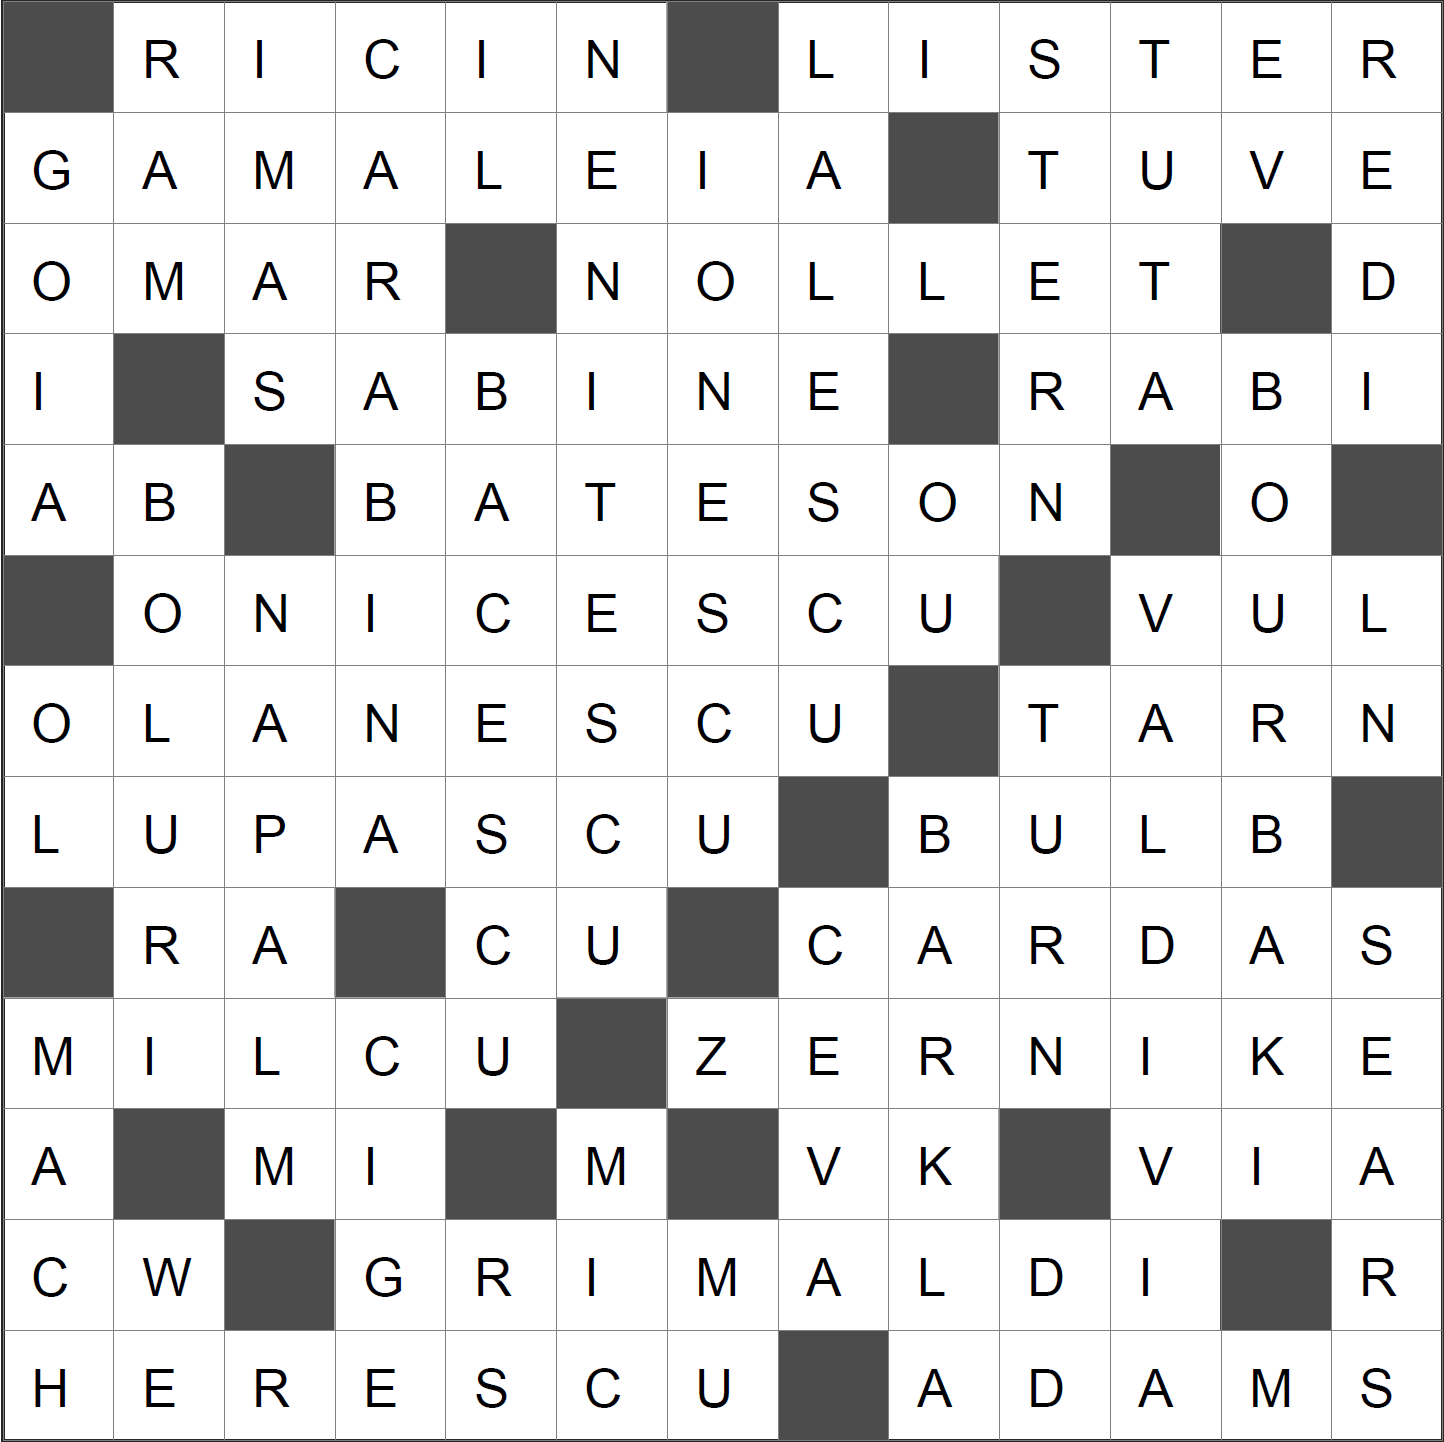
\includegraphics[width=\columnwidth]{figs/2013b.png}
\end{columns}
\end{frame}

%%%%%%%%%%%%%%%%%%%%%%%%%%%%%%%%%%%%%%%%%%%%%%%%%%%%%%%%%%%%%%%%%%%%%%%%%%%%%%%%

\begin{frame}{Main Contribution}

\bei

\ie \tcm{AI used to lag behind the top-12 scores~[\cite{DBLP:conf/cig/BulitkoB21}]}

\bigskip

\bigskip


\ie \tcg{Our approach entered top-12 range in each of the three years tried}

\eei

\end{frame}


%%%%%%%%%%%%%%%%%%%%%%%%%%%%%%%%%%%%%%%%%%%%%%%%%%%%%%%%%%%%%%%%%%%%%%%%%%%%%%%%

\begin{frame}{Related Work}

\bei

\ie \tcm{Adi: please write, use {\tt [$\backslash$cite]} for citations}

\eei

\end{frame}


%%%%%%%%%%%%%%%%%%%%%%%%%%%%%%%%%%%%%%%%%%%%%%%%%%%%%%%%%%%%%%%%%%%%%%%%%%%%%%%%


\begin{frame}{Our Approach: Overview}

\begin{columns}
\column{0.7\linewidth}

\ben
\ie build cores from a pattern (human input)

\medskip

\ie build expanded cores

\medskip

\ie build seeds

\medskip

\ie develop seeds into full solutions
\ben
\ie select promising seeds 
\ie complete them to full grids filled with words
\een
\een

\column{.3\linewidth}

\begin{figure}
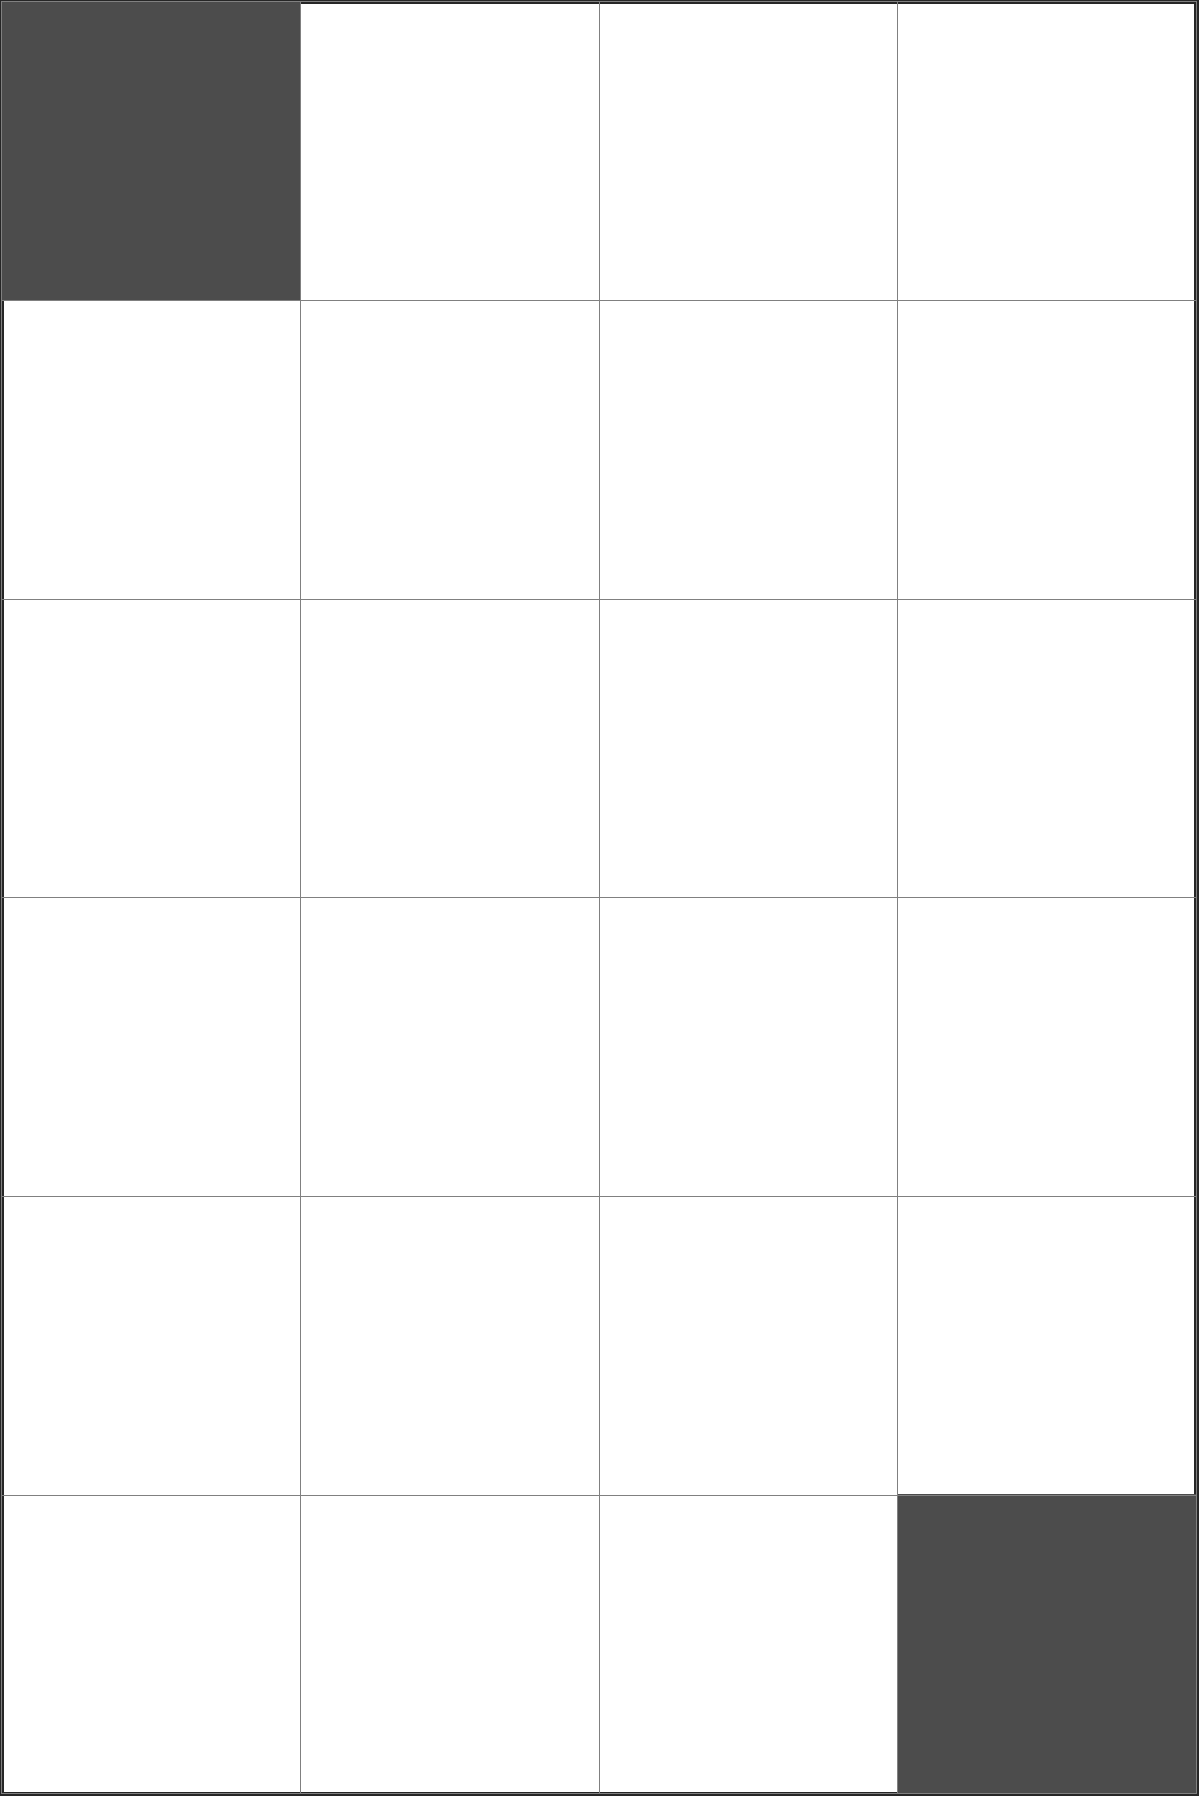
\includegraphics[width=0.7\columnwidth]{_plots/6x4-puzzle.png}
\vspace{-0.25cm}
\caption{{\bf pattern}: a rectangular grid with no letters}
\end{figure}

\end{columns}

\end{frame}

%%%%%%%%%%%%%%%%%%%%%%%%%%%%%%%%%%%%%%%%%%%%%%%%%%%%%%%%%%%%%%%%%%%%%%%%%%%%%%%%


\begin{frame}{Cores}

\begin{columns}
\column{0.7\linewidth}

\bei
\ie construct a small puzzle
\bei 
\ie the grid is the pattern
\eei

\bigskip

\ie feed the puzzle into {\sc Wombat}~[\cite{DBLP:conf/socs/BoteaB21}]
\bei 
\ie the dictionary contains substrings of thematic words
\ie generate multiple solutions 
\ie each solution is the core
\eei
\eei

\column{.3\linewidth}

\begin{figure}
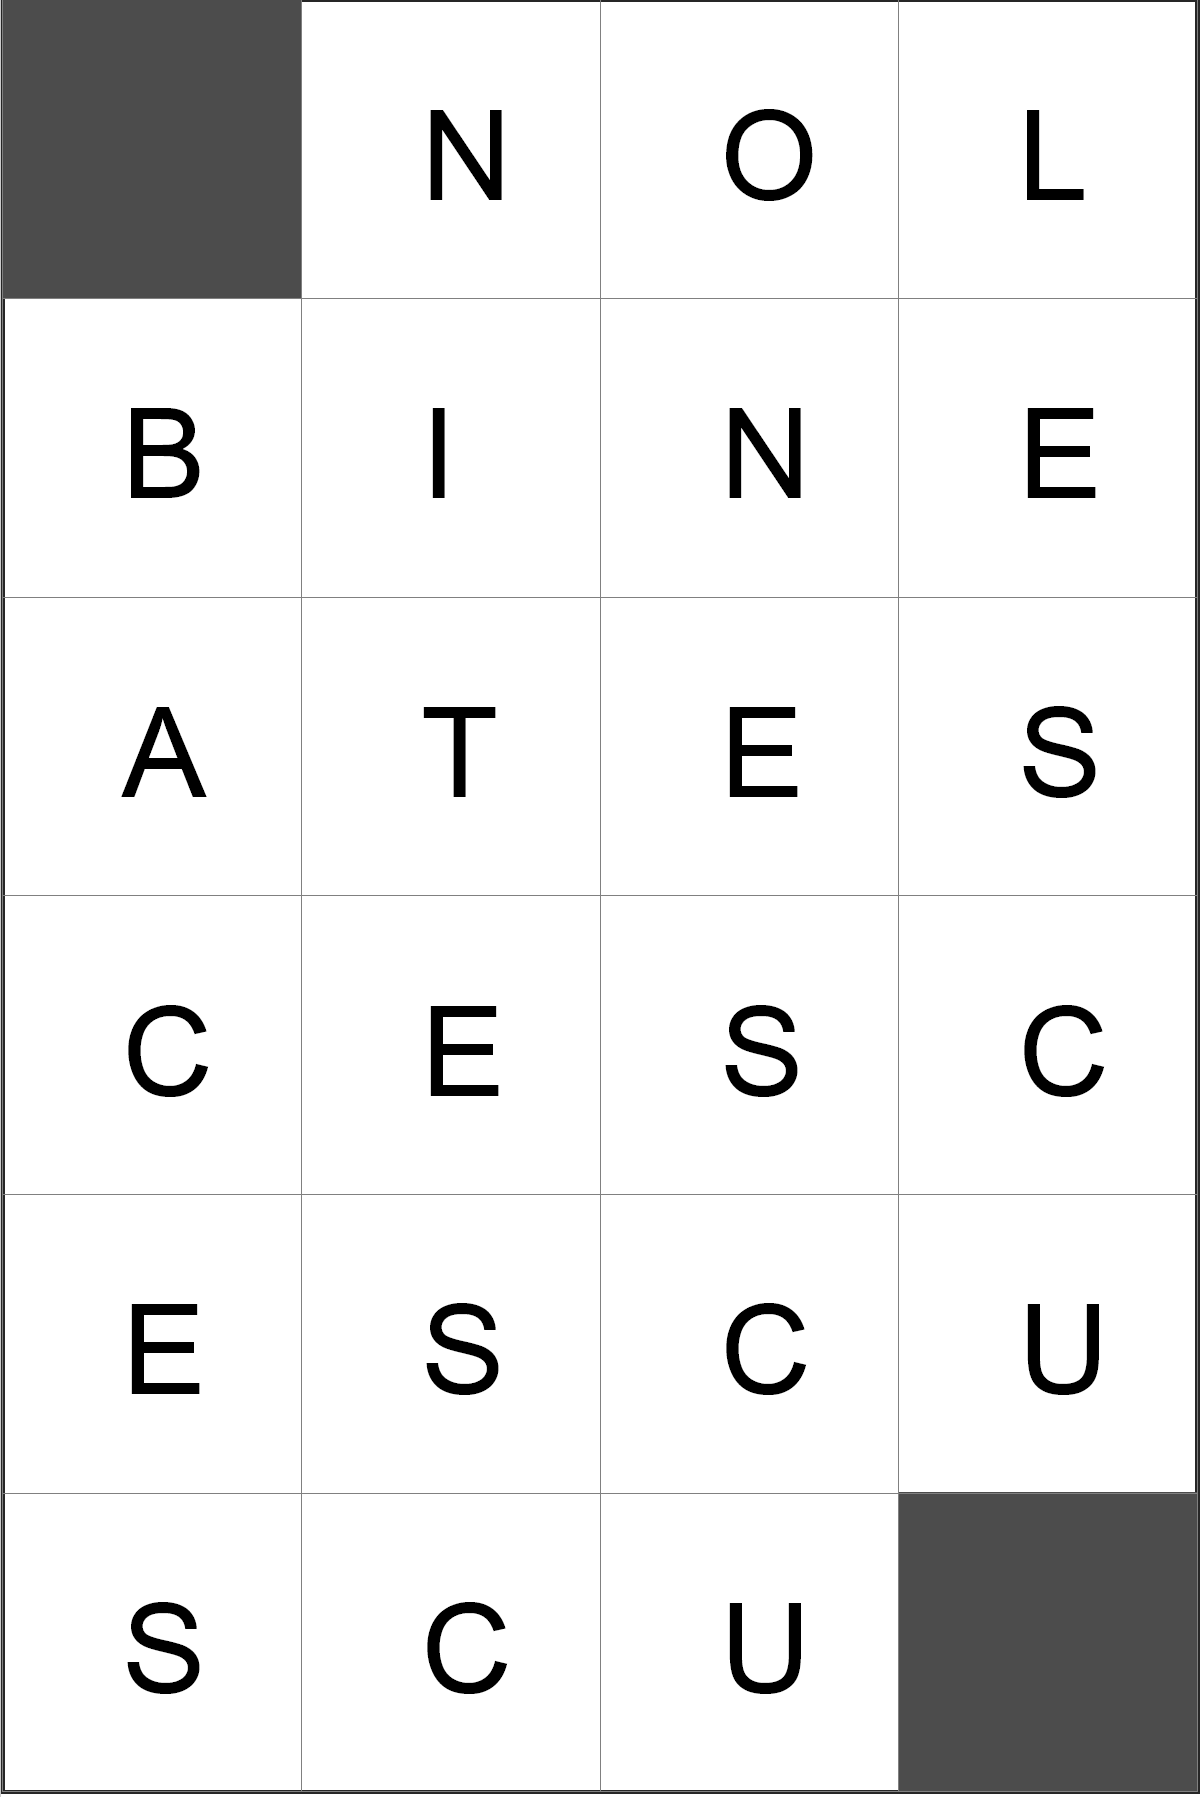
\includegraphics[width=0.7\columnwidth]{_plots/core-6x4-puzzle.png}
%\vspace{-0.15cm}
\caption{{\bf core}: a pattern filled with letters. Each word is a substring of a thematic word}
\end{figure}

\end{columns}

\end{frame}

%%%%%%%%%%%%%%%%%%%%%%%%%%%%%%%%%%%%%%%%%%%%%%%%%%%%%%%%%%%%%%%%%%%%%%%%%%%%%%%%


\begin{frame}{Expanded Cores}

\begin{columns}
\column{0.5\linewidth}

\bei
\ie match full thematic words to strings in the core
\ie depth first search \tcm{Adi: need more here}
\eei

\column{.5\linewidth}

\begin{figure}
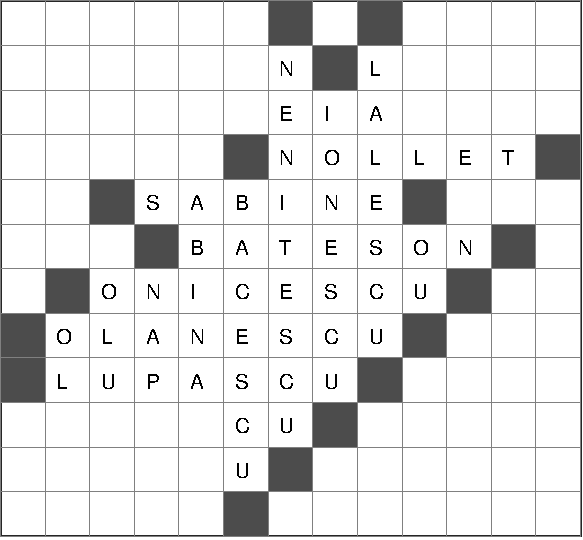
\includegraphics[width=\columnwidth]{_plots/extcore-alive-0-puzzle-72-2975-1488--1--1.pdf}
%\vspace{-0.15cm}
\caption{{\bf expanded core}: a rectangular grid with white cells, black cells and white cells with letters. Contains full thematic words bookended with black cells}
\end{figure}

\end{columns}

\end{frame}

%%%%%%%%%%%%%%%%%%%%%%%%%%%%%%%%%%%%%%%%%%%%%%%%%%%%%%%%%%%%%%%%%%%%%%%%%%%%%%%%


\begin{frame}{Seeds}

\begin{columns}
\column{0.5\linewidth}

\begin{block}{Definition}
A \emph{seed} is a full-size $13\times13$ grid with white cells, black cells, and white cells with letters.
\end{block}
\begin{block}{Building seeds from an expanded core}
\bei
\ie Place the expanded core inside the $13\times13$ grid
\ie Shift horizontally and vertically to obtain multiple seeds
\ie Prune away seeds proven illegal
\eei
\end{block}

\column{.5\linewidth}
\centering
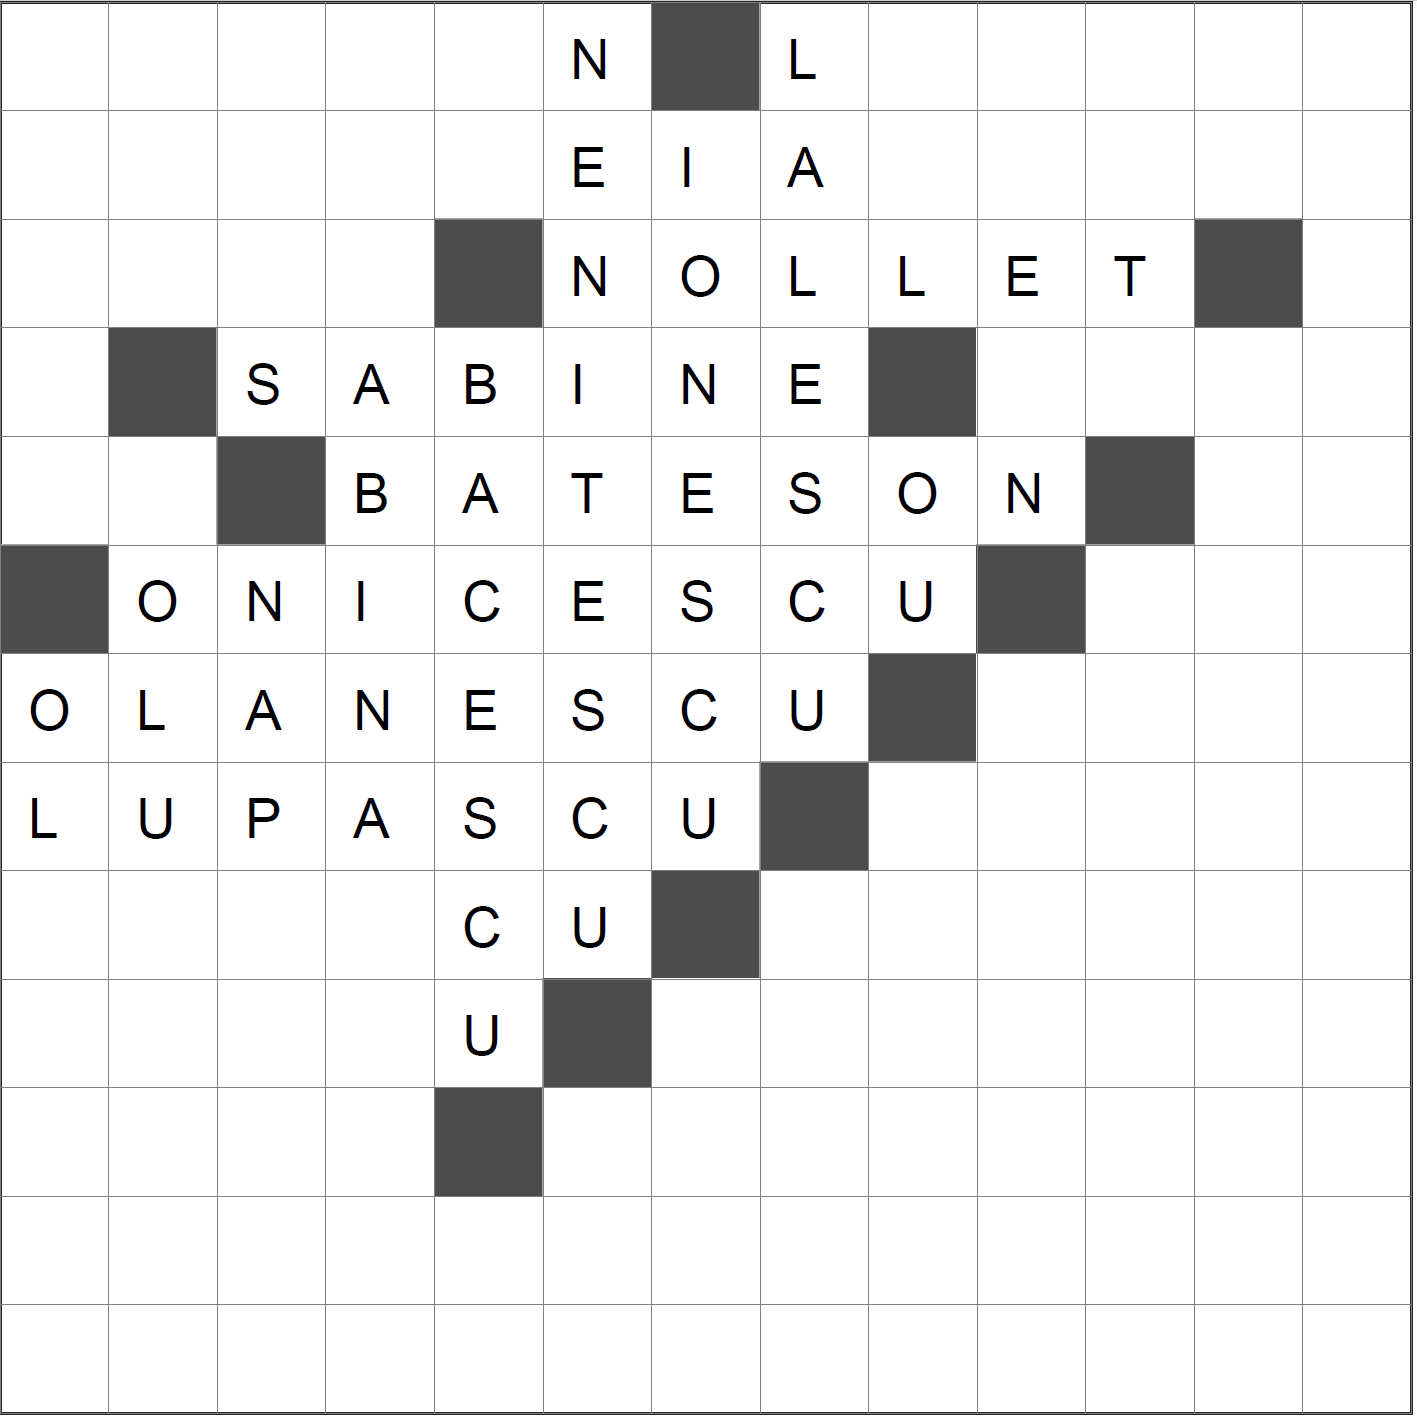
\includegraphics[height=6cm]{_plots/alive-0-puzzle-72-2975-1488--1--1.png} \hspace{1cm}
\end{columns}

\end{frame}

%%%%%%%%%%%%%%%%%%%%%%%%%%%%%%%%%%%%%%%%%%%%%%%%%%%%%%%%%%%%%%%%%%%%%%%%%%%%%%%%


\begin{frame}{Example with Building a Seed}

\begin{figure}
\centering
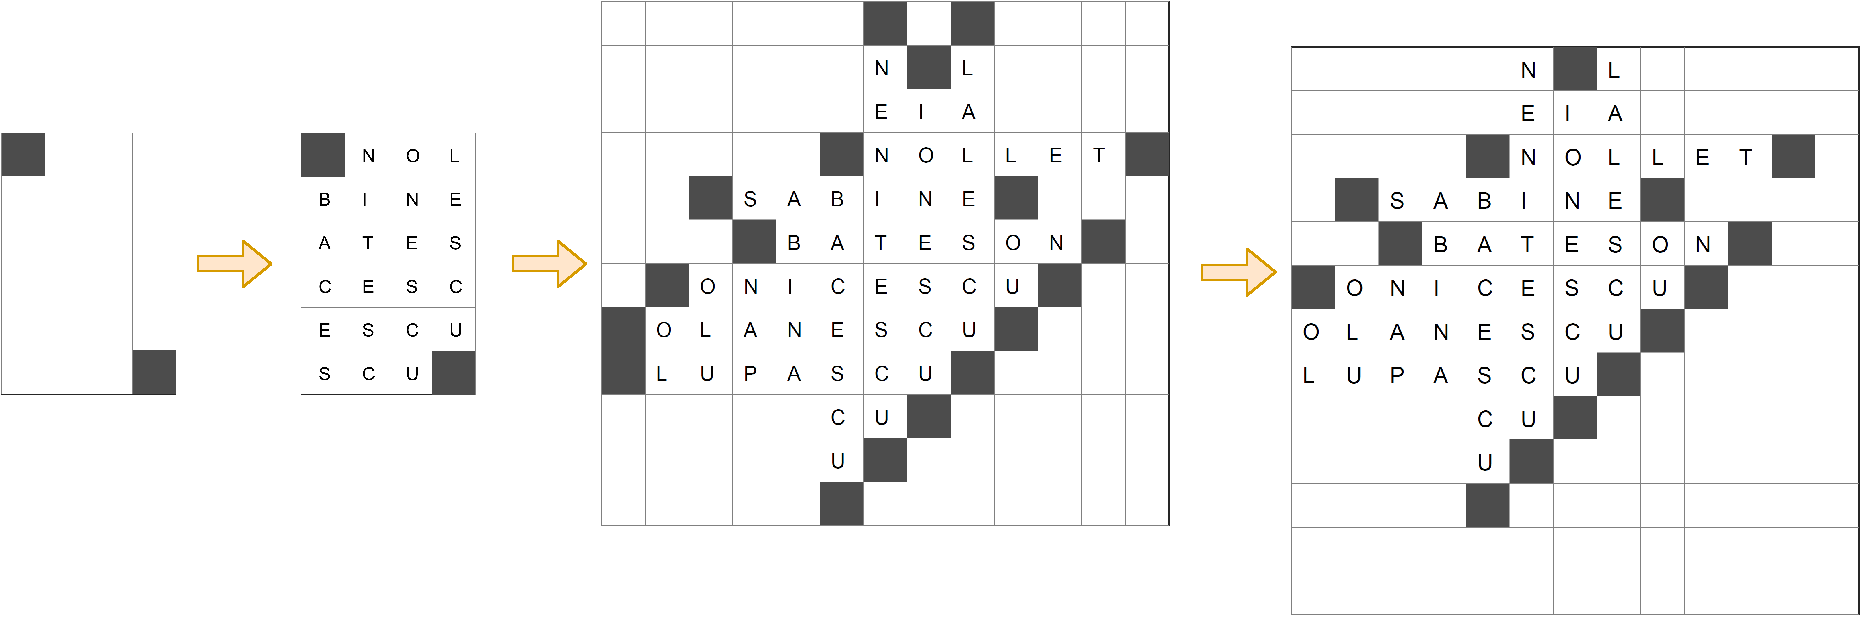
\includegraphics[width=\textwidth]{figs/4part.pdf}
\caption{Gradually building a seed: pattern $\rightarrow$ core $\rightarrow$ expanded core $\rightarrow$ seed. The different stages of the build are aligned vertically to illustrate how the expansion and build happen. Note, for instance, how the partial word ``NOL'' becomes ``NOLLET''. }
\label{fig:pattern}
\end{figure}

\end{frame}


\begin{frame}{Conclusions}


\end{frame}

%%%%%%%%%%%%%%%%%%%%%%%%%%%%%%%%%%%%%%%%%%%%%%%%%%%%%%%%%%%%%%%%%%%%%%%%%%%%%%%%

\begin{frame}[allowframebreaks]{Bibliography}
\renewcommand*{\bibfont}{\footnotesize}
\printbibliography
\end{frame}

%%%%%%%%%%%%%%%%%%%%%%%%%%%%%%%%%%%%%%%%%%%%%%%%%%%%%%%%%%%%%%%%%%%%%%%%%%%%%%%%

\end{document}



